% Chapter X

\chapter{Infection of \textit{Acanthamoeba castellanii} by \textit{Legionella pneumophila}} % Chapter title

\label{ch:02-02} % For referencing the chapter elsewhere, use \autoref{ch:name} 

%----------------------------------------------------------------------------------------

\textit{Legionella pneumophila} alters its host signal transduction, metabolism and gene regulation upon infection. In addition to all these changes, it also affects host histone marks, which are known to be related to gene regulation and genome architecture. In this chapter, we investigate the genome structure of the amoeba \textit{A. castellanii}, a natural host of \textit{L. pneumophila}, and how it is affected during infection by the bacterium.

Several strains of \textit{A. castellanii} have been isolated throughout history.These strains may originate from different ecological niche of geographical location and have been cultivated in labs for long preriods. As a result, they can differ in various phenotypes, including susceptibility to infection. Comparing such divergent strains can also help us understand what genomic features are important for pathogen susceptibility.

As with most other genomics techniques, a prerequisite of Hi-C analyses is to have a high quality reference genome with clearly delimited chromosomes. At the time of writing, the A. castellanii reference genome is split into 3192 contigs merged into 384 scaffolds which do not represent chromosomes.

This prompted us to generate a chromosome-level genome assembly for two strains of \textit{A. castellanii}: The Neff strain \cite{neffPurificationAxenicCultivation1957}, which is the reference strain for genomic analyses in that species, and the C3 strain \cite{michelIsolationAcanthamoebaStrain1997}, which is generally used for infection experiments with \textit{L. pneumophila} due to higher infection rates. In the following manuscript, we describe and compare the genomic landscape of both strains, as well as the spatial organization of their genomes. We also investigate changes happening in the 3D genome organization in response to infection by \textit{L. pneumophila}.

\includepdf[pages=-,addtotoc={
     1,section,1,Regulation of the \textit{A. castellanii} genome upon infection,p1,
     1,subsection,2,Introduction,p2,
     2,subsection,2,Results,p3,
     7,subsection,2,Discussion,p4,
     7,subsection,2,Methods,p5}]
     {Publications/acastellanii_legionella_manuscript.pdf}    


\section{Inter-strain sequence divergence}

To put into perspective the divergence between \textit{A. castellanii} strains Neff and C3, here we compare them to 11 other amoeba species whose genomes are available. As described in the previous section, we extracted all predicted coding sequences from each species and used orthofinder (v2.3.3) to constitute groups of orthologous genes among these proteomes.

We built a phylogenetic tree using orthofinder built-in implementation of the STAG (Species Tree inference from All Genes) procedure \cite{emmsSTAGSpeciesTree2018}. Briefly, Orthofinder builds a tree for each gene based on multiple sequence alignment, and then uses all gene trees where all species are available to build a species tree. C3 and Neff are highly divergent from the closest available relative, Planoprotostelium fungivorum (Fig. \ref{fig:02-02:acas-comp}a). Both strains exhibit a high (protein) sequence divergence, with about 0.084 amino-acid substitution per site, compared to e.g. 0.061 between \textit{Entamoeba histolytica} and \textit{Entamoeba dispar}. When computing the DNA sequence divergence between the two strains, we observe an average of 6.65\% substitions across aligned blocks (Fig. \ref{fig:02-02:acas-div}). In comparison, computing this same metric between Neff and \textit{Dictyostelium discoideum} yields 11.8\%.

As mentioned earlier, a high number of orthogroups are specific to either \textit{A. castellanii} strains (Fig. \ref{fig:02-02:acas-comp}b), further emphasizing their strong differences. There also seems the ba a few major genomic rearrangements between the two strains, however it is hard to assess whether these are genuine inter-strain differences. These segments could also be the product of misassemblies induced by the collapse of heterozygous structural variants in either strains.



\begin{figure}[htb]
    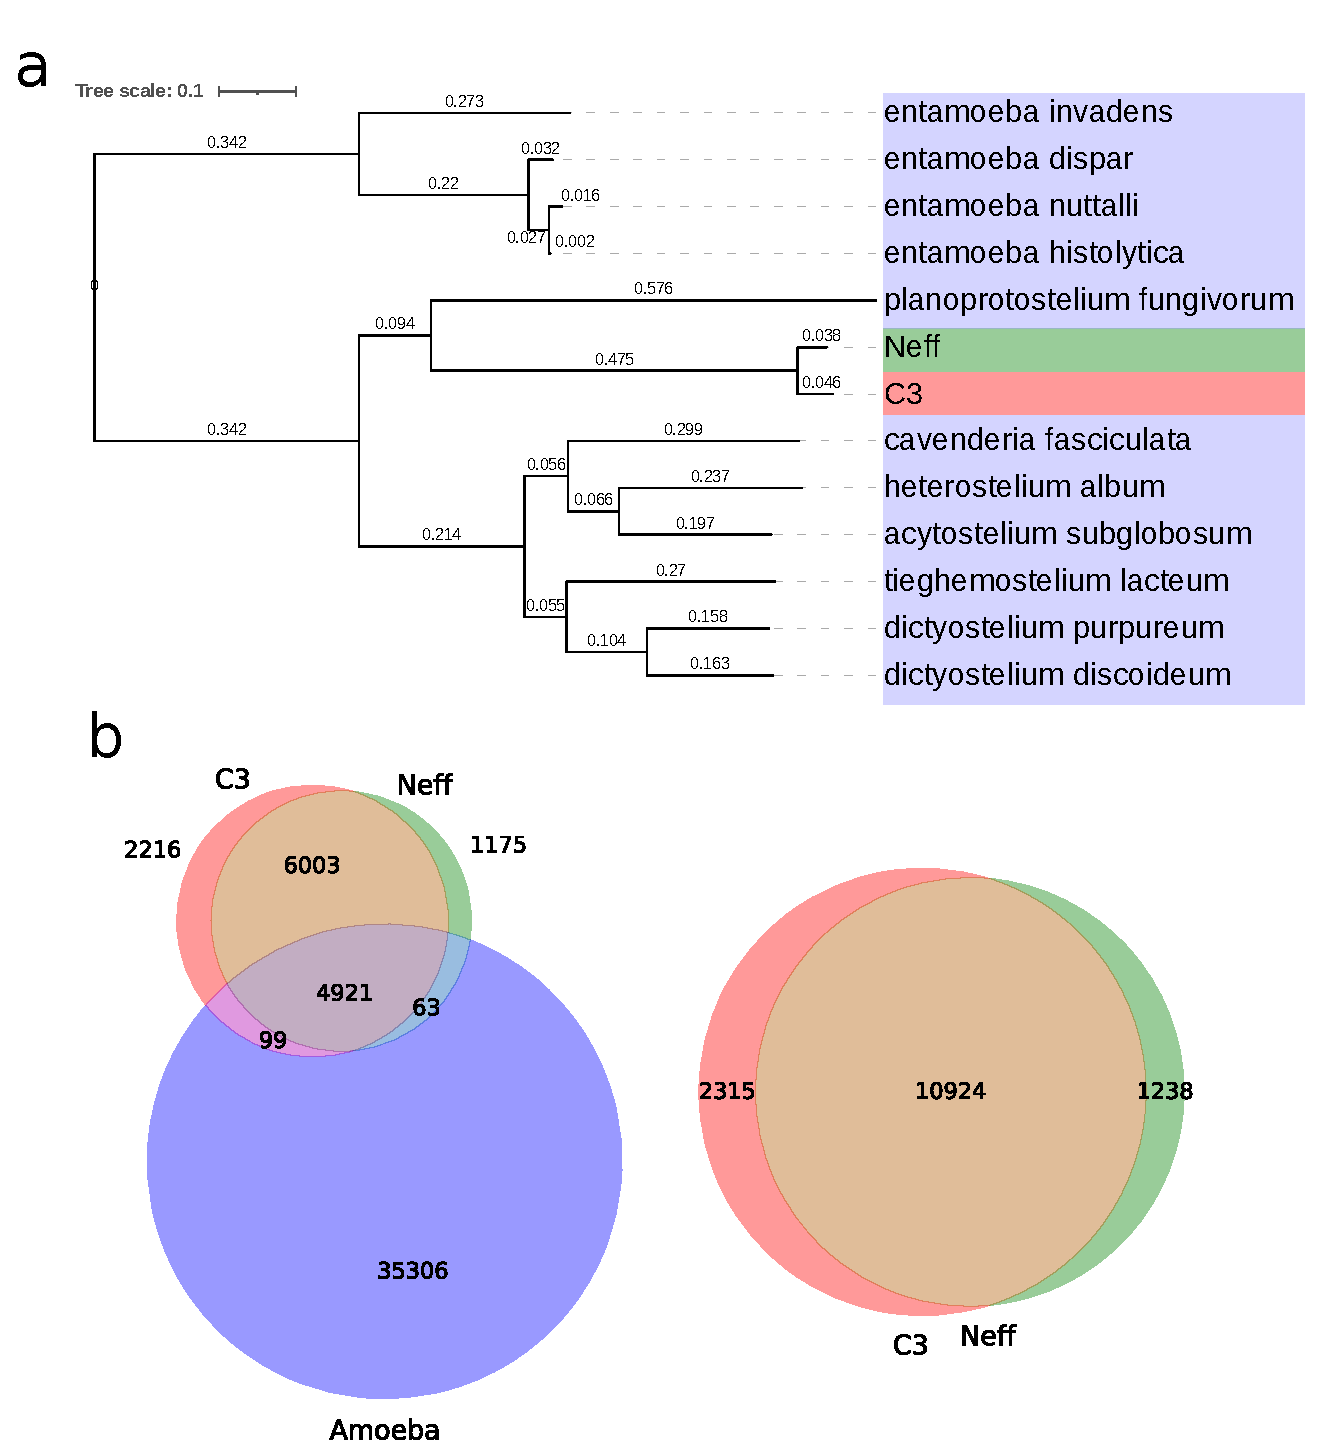
\includegraphics[width=\textwidth]{Parts/Part02/gfx/acas_comparative_genomics.pdf}
    \caption[Comparative genomics of \textit{A. castellanii}.]{Comparison of \textit{A. castellanii} strains C3 and Neff with other species. \textbf{a:} Phylogenetic tree of \textit{A. castellanii} strains C3 and Neff and 11 other amoeba species built based on all coding sequences. Distances represent substitution per position. \textbf{b:} Comparison of orthogroups content between \textit{A. castellanii} and the 11 other amoeba species used in the tree.}
    \label{fig:02-02:acas-comp}
\end{figure}

\begin{figure}[htb]
    \center
    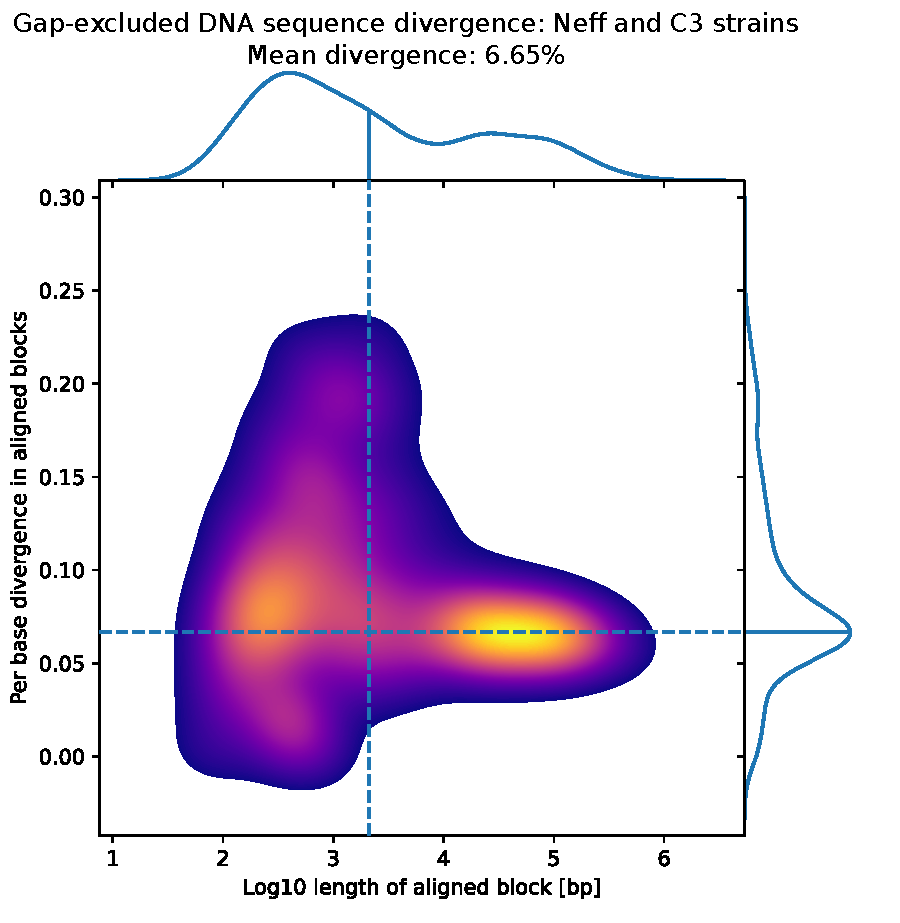
\includegraphics[width=0.8\textwidth]{Parts/Part02/gfx/acas_strains_div.pdf}
    \caption[Sequence divergence between \textit{A. castellanii} strains C3 and Neff.]{Density plot showing the distribution of sequence (gap-excluded) divergence across aligned blocks between \textit{A. castellanii} strains C3 and Neff.}
    \label{fig:02-02:acas-div}
\end{figure}

\begin{figure}[htb]
    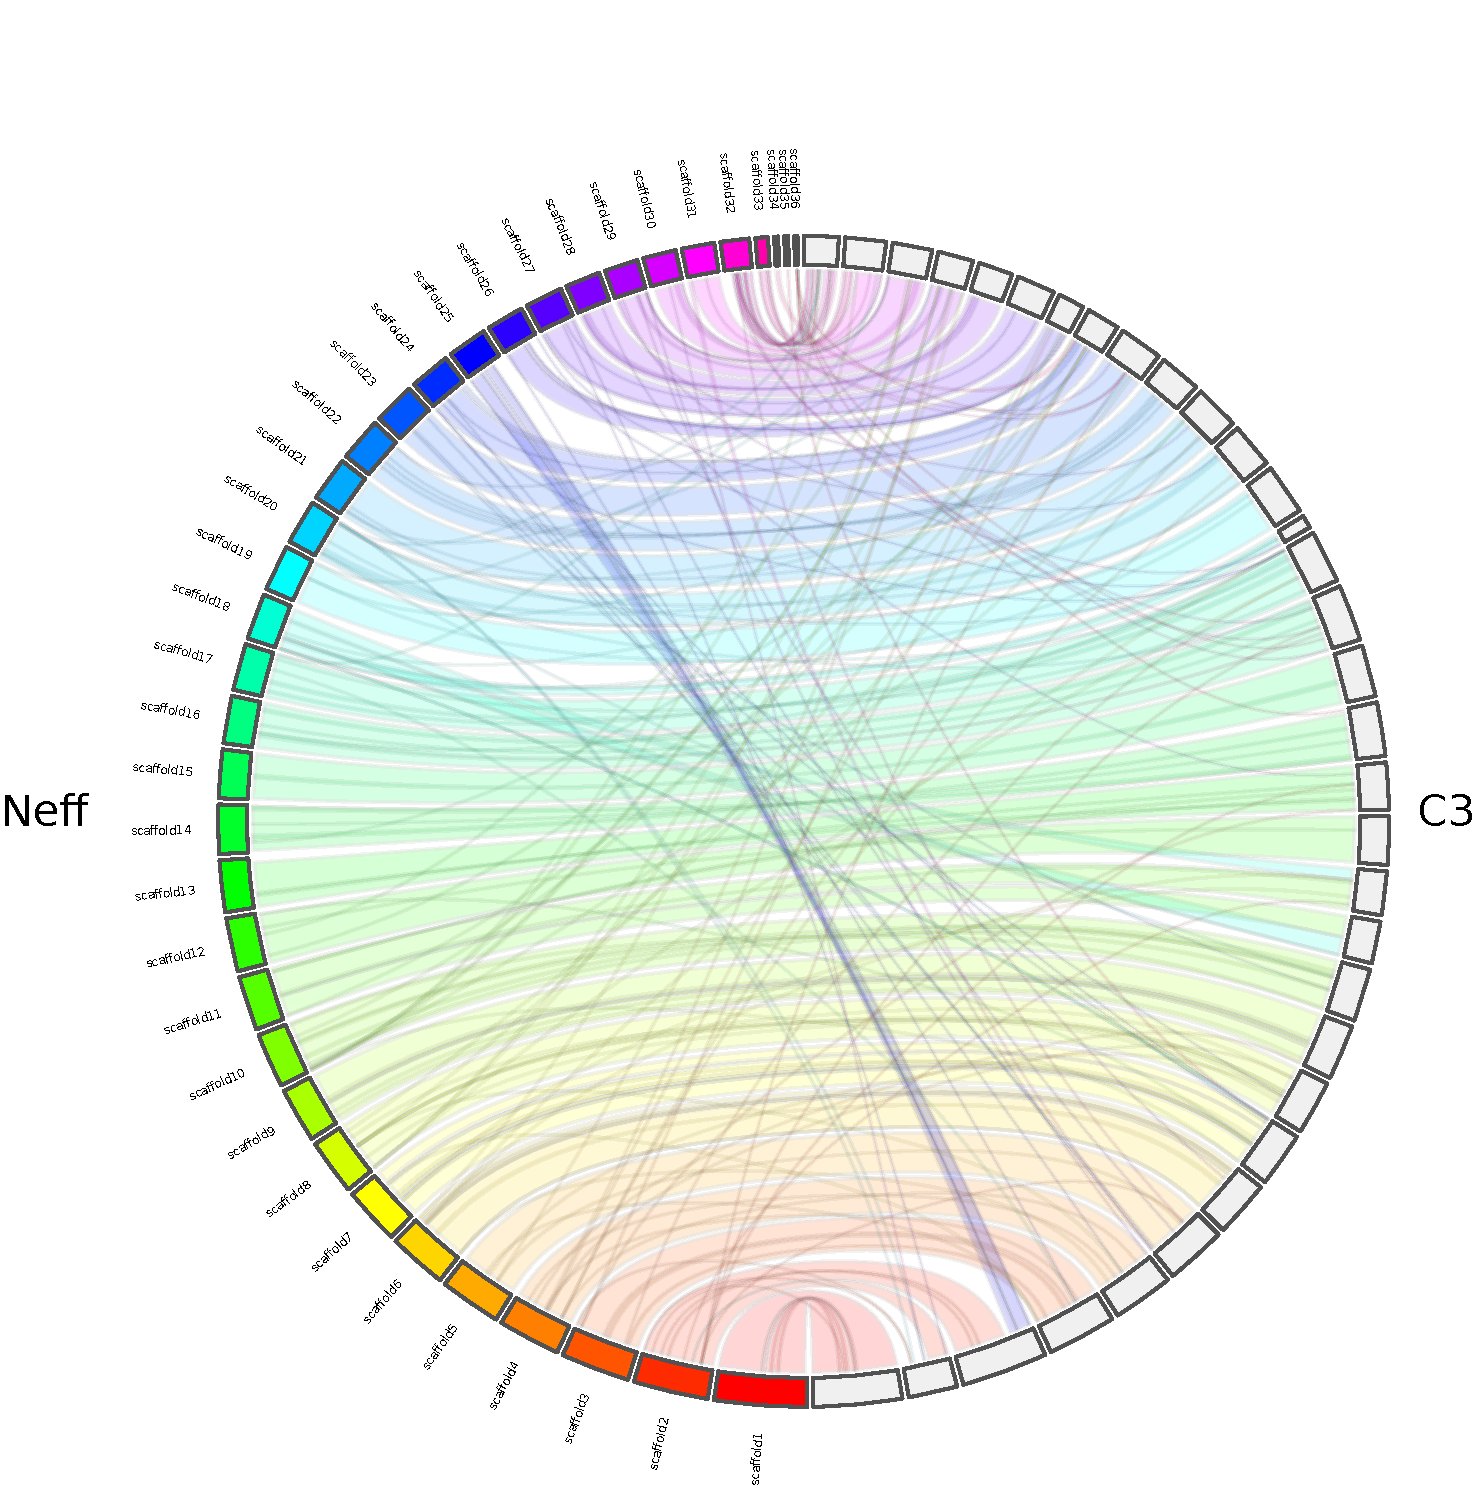
\includegraphics[width=\textwidth]{Parts/Part02/gfx/acas_circos.pdf}
    \caption[Circos plot of \textit{A. castellanii} strains C3 and Neff.]{Circos plot showing homologous blocks for all scaffolds of \textit{A. castellanii} strains C3 and Neff longer than 50kb.}
    \label{fig:02-02:acas-circos}
\end{figure}
